\documentclass{beamer}

\usepackage[utf8]{inputenc}
\usepackage{default}
\usepackage{pdfpages}


\begin{document}

\begin{frame}
\textbf{Homework\\}
Draw an unrooted tree from the table of splits shown on the next page.
The frequencies shown in the table represent bootstrap proportions. 
Numbers at the top are taxon labels from 01-15.
We’ll
cover bootstrapping later in the course – for now you can treat the “Freq”
column as label for the branches.\\
Start at the first row and add splits until you cannot add any more splits to
the tree.\\
Make sure to label the leaves of the tree with the taxon number and the
edges with the value found in the “Freq” column.
Upload image to catcourses.
\end{frame}

\begin{frame}
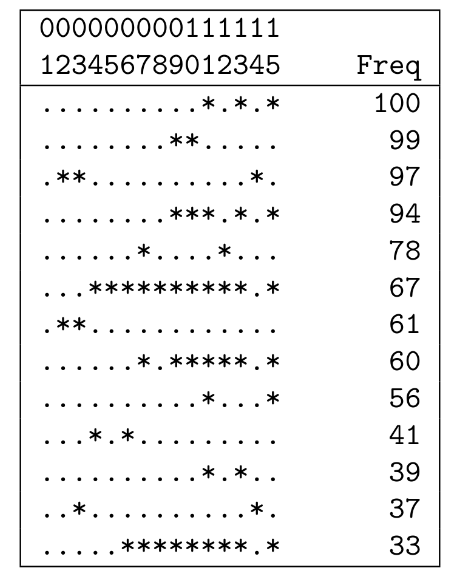
\includegraphics[width=0.5\textwidth]{splits}
\end{frame}


\end{document}
